% Chapter 7

\begin{savequote}[\quotewidth]
It is a bad plan that admits of no modification.
\qauthor{Publilius Syrus}
\end{savequote}

\chapter{Application: Modified SFC} % Main chapter title

\label{Chapter7} % For referencing this chapter elsewhere, use \ref{Chapter7}

\section{Introduction}

The previous chapter described SFC×GC runs with neat carbon dioxide as mobile
phase for the SFC separation. Carbon dioxide as a mobile phase is compatible with
a flame ionization (FID) detector: under the conditions found in the
hydrogen-rich portion of the flame the carbon dioxide cannot be reduced to
methane, the first step in the process that produces the ions that gives the FID
its name. But most modern SFC development involves the use of modifiers and
additives\footnote{Modifiers are added to the carbon dioxide to manipulate the
solubility of the analytes in the mobile phase, in exactly the same way that
mixtures of solvents are used in, say, gradient elution in HPLC. Additives are
added in small amounts, and manipulate the interaction of the analyte with the
stationary phase.}. These modifiers are usually organic compounds, and in the FID
flame they produce ions. Because the modifiers are present in much higher
quantities than the analytes, in an FID they will produce many more ions than
than the analyte, and therefore the analyte signal will be swamped by the
modifier signal. Mixing organic additives and modifiers
with the carbon dioxide mobile phase therefore renders SFC incompatible
with flame ionization as a detection method. Therefore, most modern SFC
chromatographs use optical detectors, most commonly UV spectrophotometry
borrowed from HPLC.

While the use of optical detectors have not hampered the development of SFC,
they do have a few limitations, which might be imposing artificial limits on
exploiting the versatility of carbon dioxide as a mobile phase:

\begin{itemize}

\item While SFC is compatible with optical detection (carbon dioxide is does not
absorb visible or ultraviolet radiation), there is a wide range of potential
modifiers that are not compatible with spectrophotometric detection because they
absorb strongly in the UV, but might have chemical properties useful for
manipulating SFC separations.

\item Optical detectors can only detect analytes with chromophores, and the
intensity of the signal depends strongly on the species.

\item Optical detectors have a limited dynamic range, which complicates quantification. 

\end{itemize}

In comparison, the FID can detect practically any organic compound over a wide
concentration range, giving a signal proportional to the mass of the compound.

If only there were a way to separate the the modifiers from the analytes before
detection \ldots

When GC is comprehensively coupled to SFC, the modulator will focus each
fraction of SFC eluate, and then the GC will separate all the compounds in the
fraction, analytes and modifiers included. If the modifiers are less volatile
than the analytes then the modifiers will elute before the analyte, and the
analyte can be detected or quantified using an FID, and the signal from the
modifier can be ignored.

Of course it is quite likely that the peak from the modifiers will
\keyword{overload} the GC. Both the detector and the column may be overloaded.
If the \emph{detector} is overloaded, then it just means that the detector no
longer responds linearly to the amount of material eluting from the column ---
this might include responding with its maximum output, leaving flat-topped
peaks. If the \emph{column} is overloaded, then the capacity of the stationary
phase is exceeded and the peaks will \keyword{front}: they will be asymmetrical,
with the side of the peak towards earlier elution times having a slope smaller
than the slope of non-overloaded peaks, and the side of the peak towards later
elution times having a larger slope.

The requirement that the modifiers added to the SFC mobile phase be volatile (so
that they can elute before the analyte) is not too onerous a restriction. Higher
volatility correlates with lower diffusivity, so that the preferred
high-diffusivity modifiers for SFC  would also tend to be be volatile enough to
elute early on GC. 

A practical SFC×GC chromatograph opens up the field for the use of carbon
dioxide mixed with modifier as a mobile phase for analysing complex mixtures
found in biodiesel production, biodiesel quality control, and compliance
monitoring.

\section[SFC×GC with modifier]{SFC×GC using modified carbon dioxide.}

In this section a SFC×GC chromatogram is presented that shows that methanol
added as a modifier to the SFC mobile phase does not interfere with the fast GC
any more than a sample's solvent interferes in the usual 1D GC. The 2D
separation space of SFC×GC therefore gains in control over elution in the SFC
dimension at the cost of losing the capability to detect compounds
more volatile than methanol on the GC dimension.

\subsection{Sample}

The sample was a 1:1 blend of petrodiesel and biodiesel, prepared in the
laboratory. The biodiesel sample was donated by a commercial testing laboratory,
and had been produced from palm oil by an anonymous producer. The petrodiesel
(Shell Extra Diesel 500 ppm) was obtained from a commercial filling station.

\subsection{SFC}

The SFC used carbon dioxide at \SI{200}{\bar} inlet pressure and room
temperature as mobile phase. The flow rate is of carbon dioxide at atmospheric
pressure was reportedly \SI{175}{\milli\litre\per\minute}. The carbon dioxide
mobile phase was modified with \SI{5}{\percent} mass fraction of HPLC-grade
methanol (Merck LiChrosolv). The column consisted of five HPLC bare silica
columns (150 mm $\times$ 4.6 mm, 3 $\mu$m particles) (Restek, Pinnacle DB
Silica) connected in series.

\subsection{Modulation}

A fraction was collected for each \SI{5}{\second} SFC flow time. After the flow
from the SFC was stopped, \SI{3}{\second} was allowed for the last vapour in the
inlet to be swept into the cold (\SI{-20}{\celsius}) column for trapping, and
then the inlet vent valve was opened for \SI{1}{\second} to relieve excess inlet
pressure.

\subsection{GC}

The GC column was a Restek Rxi-5Sil MS \SI{0.250}{\milli\metre} x
\SI{0.25}{\micro\meter} × \SI{1}{\metre}. The hydrogen carrier gas flowed at a
rate of \SI{11.6}{\milli\litre\per\minute}.

For each fast GC program the temperature was ramped from \SI{-20}{\celsius} to
\SI{320}{\celsius} in \SI{10.3}{\second} (\SI{33}{\celsius\per\second}) and kept
there for \SI{10}{\second} before cooling the column down to \SI{-20}{\celsius}
again, in preparation of trapping the next fraction.

A total of 233 fast chromatograms were recorded and combined into a 2D
chromatogram.

\subsection{Results and discussion}

The chromatogram obtained for this run is shown in Figure \ref{fig:Modifier}.
Note the unusual orientation of the chromatogram, chosen to best show the data:
In the SFC dimension the later elution times are closer to the reader.

\begin{figure}
	\centering
	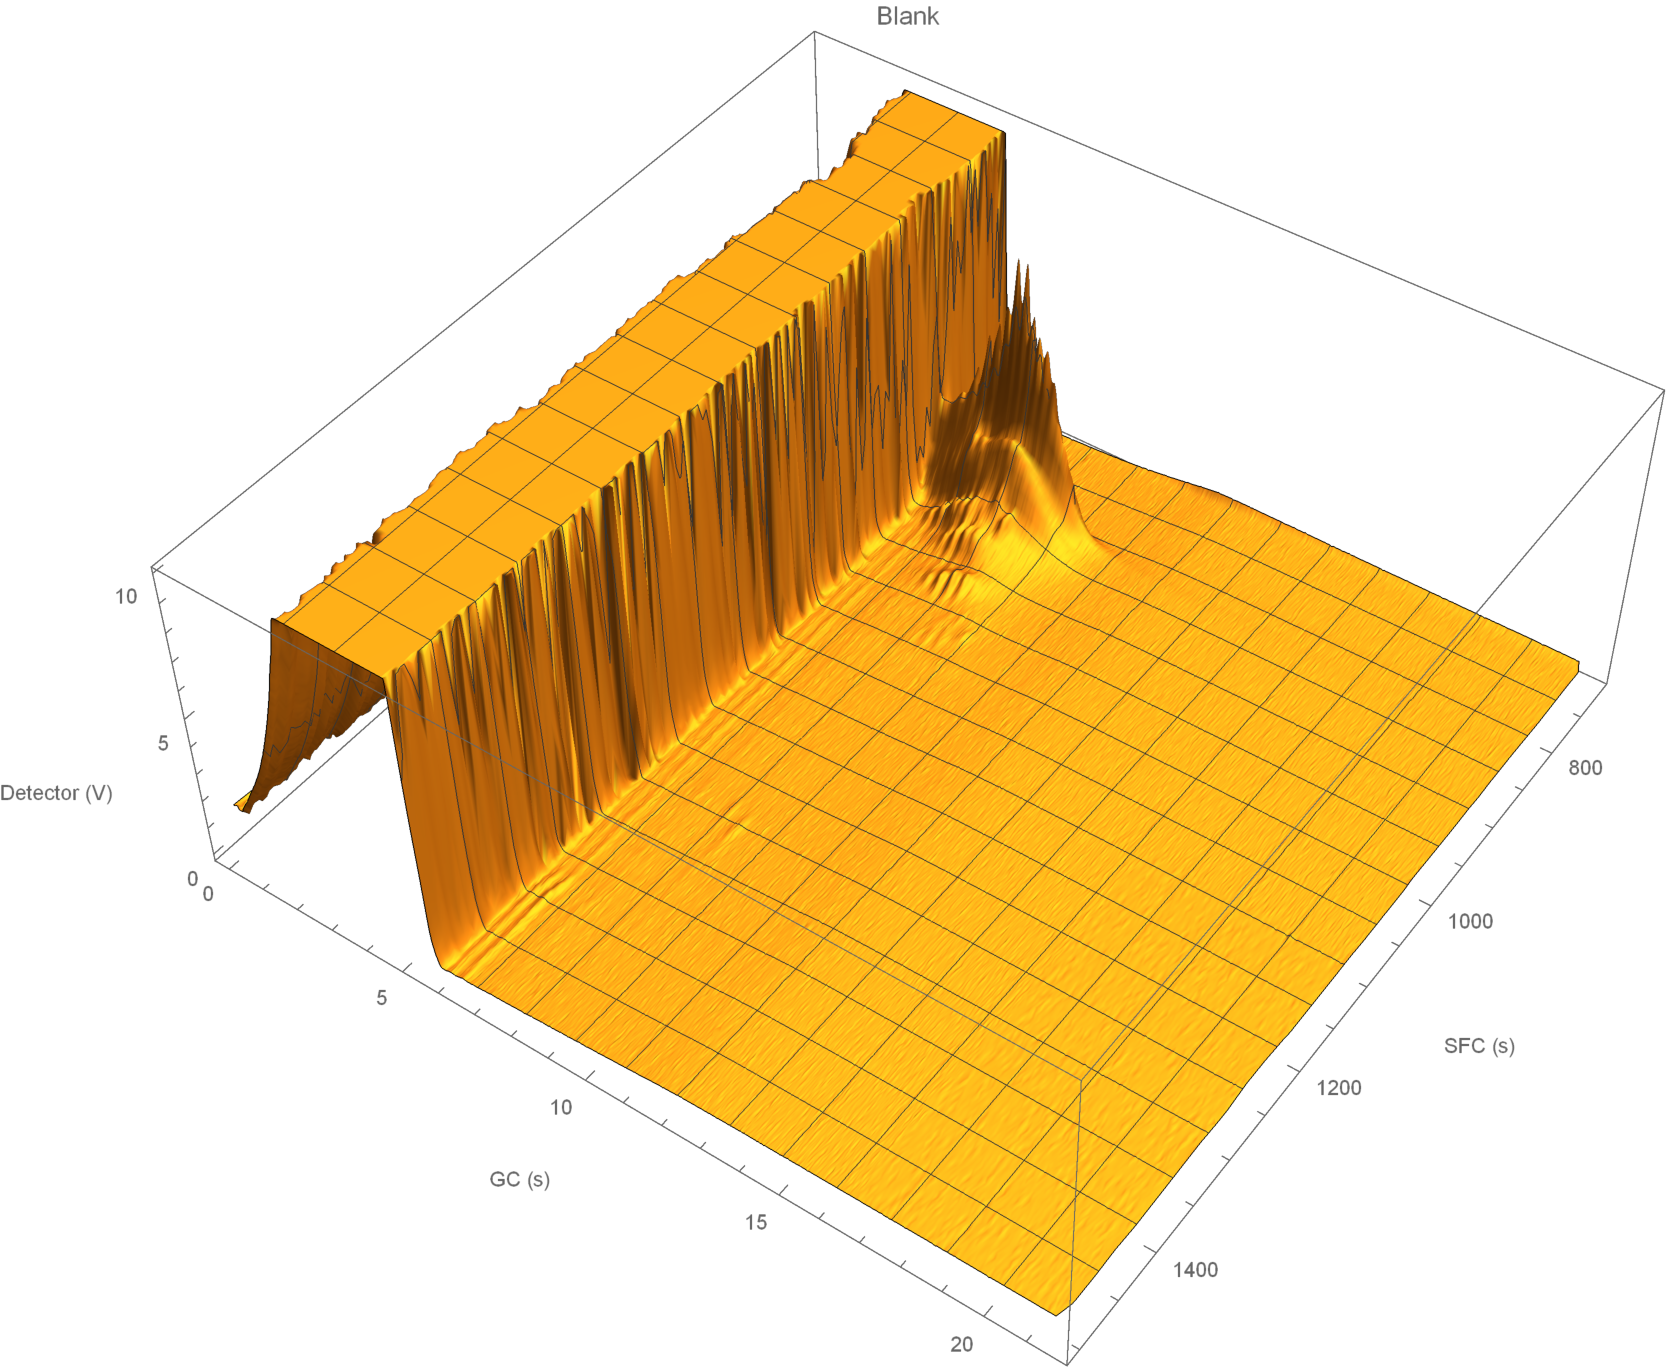
\includegraphics[width=\textwidth]{Figures/Modifier.pdf}
	\decoRule	
	
	\caption[Modifiers in SFC]{The modifiers used in the SFC dimension elutes as a
solvent front on the GC dimension, and does not otherwise affect the separation.}
	
	\label{fig:Modifier} 
\end{figure}

The intention of this chromatographic run was to explore the effect of the
meth\-anol modifier on the retention behaviour of the biodiesel fraction of the
B50 blend. However, the run time was not long enough for the FAMEs to elute and
the only peaks on the chromatogram are the group of hydrocarbons from the
petrodiesel. Nevertheless, the chromatogram shows the possibilities that arise
when a modifier is added to the SFC mobile phase.

The 'wall' that appears on the chromatogram is the tailing edge of the peak of
the modifier added to the SFC. These peaks are present in all the fractions at
equal concentrationa. The flat top of the peak is caused by detector overload. 

It should be noted that the detector overload is not caused by saturation of the
FID response, but by the limits imposed by the chosen signal amplifier. The FID
has a dynamic range of 10\textsuperscript{6}, and could comfortably accommodate
the modifier peak, but the amplifier gain was chosen to best match the analyte signal
with the input range of the 16-bit analog-to-digital converter.

The 'corrugations' on the wall can be ascribed to two sources. First is
variations in retention time of the modifier peak, which can be caused by
variations in GC gas flow and variations in the fast temperature programs.
Second, variations in the amount of modifier collected by the modulator will
also cause slight changes in the apparent position of the peak. This second
reason is probably the major contributor for this run, caused by variations in
the timed collection period introduced by the imprecision of the
electromechanical valve actuator and by variations in the SFC flow.

The chromatogram shows the hydrocarbon ``hump'' in the GC dimension and the
separation of the aromatics in the SFC dimension, as discussed in Section
\ref{sec:B50Discuss}. It can be seen that the 'solvent peak' of the modifier
interferes with the more volatile of the hydrocarbons, but the rest of the
separation space is available for separation. 

\subsection{Conclusion}

Adding modifiers to SFC expands the versatility of carbon dioxide as a mobile
phase, but in 1D SFC the use of modifiers precludes the use of the universal
flame ionization detector (FID), because the modifier signal will swamp the
analyte signal.

Adding GC-FID as a \textsuperscript{2}D separation allows the use of any
volatile modifier to manipulate retention in the SFC dimension, including
modifiers that might not be UV-transparent. Modifiers present in the fraction
collected by the modulator elute like the customary solvent peak in the GC
dimension, which means that the signal from the modifier does not interfere with
the signal of the analyte.

The example shown above shows that SFC×GC will reliably separate any modifiers
used in the SFC dimension from the analytes, allowing the FID to be used as a
detector for gradient-elution SFC separations.

